%!TEX program = xelatex
% 完整编译: xelatex -> bibtex -> xelatex -> xelatex
\documentclass[lang=cn,11pt,a4paper,cite=numbers]{elegantpaper}
\usepackage{xfp}
\usepackage{tikz}

\title{A Neural Network Model with Gap Junction for Global Feature Extraction}
\author{郑晖}
% \institute{}

% \version{0.09}
\date{\zhtoday}

% 本文档命令
\usepackage{array}
\newcommand{\ccr}[1]{\makecell{{\color{#1}\rule{1cm}{1cm}}}}

\begin{document}

\maketitle

\begin{abstract}
A Neural Network Model with Gap Junction for Global Feature Extraction.
\keywords{Gap Junction, Global Feature Extraction}
\end{abstract}

\section{Introduction}

\section{Materials \& Methods}
  我们考虑一维环状网络模型\ref{fig:network-model},该网络在E/I平衡网络\cite{van1996chaos}之上修改而来。在这个一维环状网络中,E型神经元和I型神经元分别被用来建模ipRGC和PAC。
\begin{figure}[!htb]
    \begin{center}
    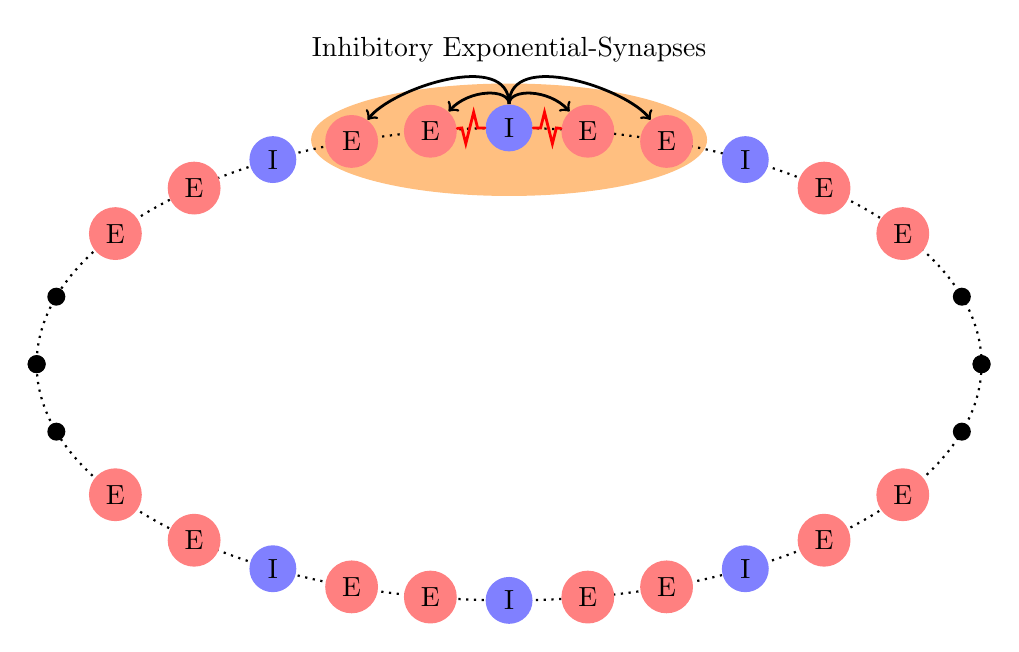
\begin{tikzpicture}
        % parameter n
        \draw[thick, fill, orange!50] (0,2.85) ellipse [x radius=2.5, y radius=0.7];

        % baseline
        \draw[thick, dotted, black] (0,0) ellipse [x radius=6, y radius=3];

        % node
        \foreach \x in {-3,0,3} {
            \node[circle, fill=blue!50] (node_{\x}_1) at (\x, \fpeval{sqrt(9*(1-(\x*\x)/36))}){I};
            \node[circle, fill=blue!50] (node_{\x}_0) at (\x, \fpeval{-sqrt(9*(1-(\x*\x)/36))}){I};
        }
        \foreach \x in {-5,-4,-2,-1,1,2,4,5} {
            \node[circle, fill=red!50] (node_{\x}_1) at (\x, \fpeval{sqrt(9*(1-(\x*\x)/36))}){E};
            \node[circle, fill=red!50] (node_{\x}_0) at (\x, \fpeval{-sqrt(9*(1-(\x*\x)/36))}){E};
        }
        \foreach \x in {-6,-5.75,5.75,6} {
            \draw[thick, fill, black] (\x, \fpeval{sqrt(9*(1-(\x*\x)/36))}) circle [radius=0.1];
            \draw[thick, fill, black] (\x, \fpeval{-sqrt(9*(1-(\x*\x)/36))}) circle [radius=0.1];
        }

        %% connection
        % Exponential Synapses
        \draw[line width=1,->] (node_{0}_1) ..controls(0,3.5) and (0.5,3.5).. (node_{1}_1);
        \draw[line width=1,->] (node_{0}_1) ..controls(0,4) and (1.5,3.5).. (node_{2}_1);
        \draw[line width=1,->] (node_{0}_1) ..controls(0,3.5) and (-0.5,3.5).. (node_{-1}_1);
        \draw[line width=1,->] (node_{0}_1) ..controls(0,4) and (-1.5,3.5).. (node_{-2}_1);
        \node[black] at (0,4) {Inhibitory Exponential-Synapses};
        % gap junction
        \draw[line cap=round,line width=1,-,red] (node_{0}_1)--(0.4,3)--(0.45,3.2)
            --(0.55,2.8)--(0.6,3)--(node_{1}_1);
        \draw[line cap=round,line width=1,-,red] (node_{0}_1)--(-0.4,3)--(-0.45,3.2)
            --(-0.55,2.8)--(-0.6,3)--(node_{-1}_1);
    \end{tikzpicture}
    \end{center}
    \caption{The neural network model}
    \label{fig:network-model}
\end{figure}
\subsection{Neuronal Dynamics}
  简便起见,模型中的所有神经元都使用LIF模型实现。所有神经元都接受来自外界的输入,其中I型神经元的外界输入只有双极细胞输入,而E型神经元的外界输入可以分为两部分:双极细胞输入和黑色素输入。双极细胞输入由于生物神经元结构相对黑色素输入有一定延迟,但这一点暂时没有被我们初步的模型所考虑。环上每一个神经元都与相邻的$n$个神经元形成电突触连接,每个I型神经元都与相邻的$m$个E神经元形成抑制性Exponential化学突触连接。

  I型神经元的动力学机制如下:
\begin{equation}
    {\tau}\frac{dV_{i}(t)}{dt} = -V_{i}(t) + \sum_{j \in N_{G}(i)}I_{ij}^{gap}(t) + I_{i}^{ext}(t)
\end{equation}
其中,下标$i = (1,...,N)$表示神经元的索引,$V_{i}$表示神经元的膜电位,$\tau$表示膜时间常数,$I_{ij}^{gap}$表示从神经元$j$通过gap junction传递而来的电流,$N_{G}(i)$表示与神经元$i$具备电突触连接的神经元集合,$I_{ext}$表示外部输入的刺激。无论何时$V_{i}(t)$到达一个固定的阈值$V_{th}$,神经元便会产生一个spike,然后将自身膜电位复位到$V_{rest}$并进入时长为$\tau^{arp}$的不应期。在仿真开始前,所有神经元的膜电位被随机初始化。

  E型神经元的动力学机制与I型神经元略有差异,多了来自I型神经元的抑制输入,其表达式如下:
\begin{equation}
    {\tau}\frac{dV_{i}(t)}{dt} = -V_{i}(t) + \sum_{j \in N_{G}(i)}I_{ij}^{gap}(t) - I_{i}^{chem}(t) + I_{i}^{ext}(t)
\end{equation}
其中,$I_{i}^{chem}(t)$表示神经元$i$通过抑制性化学突触接收到的电流,其他参数与I型神经元动力学机制中对应参数意义相同。

  由电突触介导的电流可以分成两部分:
\begin{equation}
    I_{ij}^{gap}(t) = I_{ij}^{gap,sub}(t) + I_{ij}^{gap,sup}(t)
\end{equation}
其中,$I_{ij}^{gap,sub}$表示阈下电流,$I_{ij}^{gap,sup}$表示阈上电流,被称作spikelet。由电突触介导的阈下电流如下:
\begin{equation}
    I_{ij}^{gap,sub} = J\left[V_{j}(t) - V_{i}(t)\right]
\end{equation}
其中,J表示耦合强度。阈上电流被假设与gap junction强度J成正比,并由spikelet因子$\gamma$缩放,其表达式如下:
\begin{equation}
    I_{ij}^{gap,sup}(t) = {\gamma}J\delta(t - t_{j}^{spike})
\end{equation}
其中,$t_{j}^{spike}$表示神经元$j$产生spike的时刻,$\gamma$量化spike对神经元膜电位增加量的贡献。

  由Exponential化学突触介导的电流动力学机制(current-based)如下:
\begin{gather}
    I_{i}^{chem}(t) = \bar{g}s_{i}(t) \\
    \frac{ds_{i}}{dt} = -\frac{s_{i}}{\tau_{decay}} + \sum_{j \in N_{C}(i)}\delta(t - t_{j}^{spike})
\end{gather}
其中,$\bar{g}$表示化学突触平均电导,$\tau_{decay}$表示衰减时间常数,$N_{C}(i)$表示与神经元$i$具备抑制性化学突触连接的神经元集合,$t_{j}^{spike}$表示神经元$j$产生spike的时刻。

  外部输入电流$I_{i}^{ext}$,携带着图像的亮度信息。其被建模为带有高斯白噪音的连续电流:
\begin{equation}
    I_{i}^{ext}(t) = \mu_{i}^{ext} + \sigma^{2}\eta_{i}(t)
\end{equation}
其中,$\mu^{ext}$是外部输入的平均值,$\sigma^{2}$是外部输入震荡的幅度,$\eta_{i}(t)$满足$\left\langle\eta_{i}(t)\right\rangle = 0$,并且$\left\langle\eta_{i}(t)\eta_{j}(t')\right\rangle = \delta_{ij}\delta(t - t')$。通常情况下,幅度$\sigma^{2}$在我们的模拟中被设为一个恒定值,大概是外部平均输入的10\%。值得注意的是,E型神经元的外部输入平均值$\mu_{E}^{ext}$略大于I型神经元的外部输入平均值$\mu_{I}^{ext}$。其原因在于E型神经元是对ipRGC进行建模,ipRGC不仅接受双极细胞的输入(PAC仅有的外部输入),还接受自身黑色素产生的感光输入。

\section{Results}
  在神经元初始化时,我们使用Gaussian随机初始化。
\subsection{PAC的抑制性化学突触近邻范围影响光自适应速度}
  在我们将es\_neighbors设置为5时,ipRGC的发放很快便被抑制,如图\ref{fig:101-es5-w3.5}。当es\_neighbors被设置为3时,ipRGC的发放会持续更长的一段时间,如图\ref{fig:101-es3-w3.5}。
\begin{figure}[!htb]
  \centering
  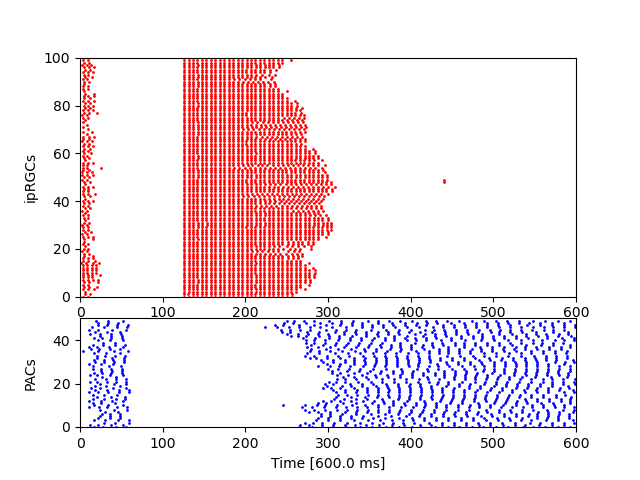
\includegraphics[width=0.6\textwidth]{figs/101-es5-w3.5.png}
  \caption{fig:101-es5-w3.5}
  \label{fig:101-es5-w3.5}
\end{figure}\begin{figure}[!htb]
  \centering
  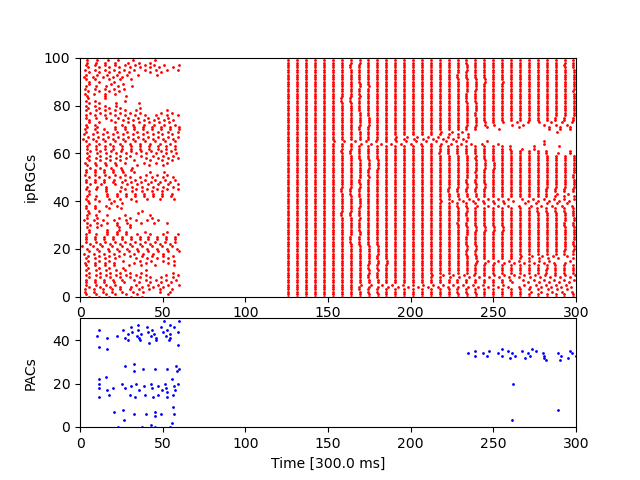
\includegraphics[width=0.6\textwidth]{figs/101-es3-w3.5.png}
  \caption{fig:101-es3-w3.5}
  \label{fig:101-es3-w3.5}
\end{figure}

% \nocite{*}
\bibliography{ref/refs}

\end{document}
